\documentclass[tikz,border=6mm]{standalone}
\usepackage{amsmath,amssymb}
\usepackage{fontspec}

\usetikzlibrary{positioning,arrows.meta,shapes.geometric,fit,backgrounds,calc}

% Master Academic Palette (WCAG AA & Color-Vision Deficiency Compliant)
\definecolor{navyblue}{RGB}{30, 60, 105}    % #1E3C69 - Model architectures, encoders, primary flows
\definecolor{tealblue}{RGB}{20, 110, 105}   % #146E69 - Data plane, ingestion, datasets, gold annotations
\definecolor{purplecat}{RGB}{95, 45, 120}   % #5F2D78 - Multi-task balancing, loss dynamics, statistics
\definecolor{ambergold}{RGB}{180, 85, 15}   % #B4550F - Hardware testbed, serving trials, embeddings
\definecolor{forestgreen}{RGB}{25, 115, 60} % #19733C - Acceptance gates, verified thresholds
\definecolor{crimsonred}{RGB}{175, 40, 40}  % #AF2828 - Feedback loops, out-of-domain holdouts, errors
\definecolor{slategrey}{RGB}{70, 85, 100}   % #465564 - Neutral boundaries, containers, baseline nodes

% Semantic aliases for architecture views
\colorlet{datagreen}{tealblue}
\colorlet{modelblue}{navyblue}
\colorlet{trainpurple}{purplecat}
\colorlet{serveorange}{ambergold}
\colorlet{logslate}{slategrey}

\begin{document}
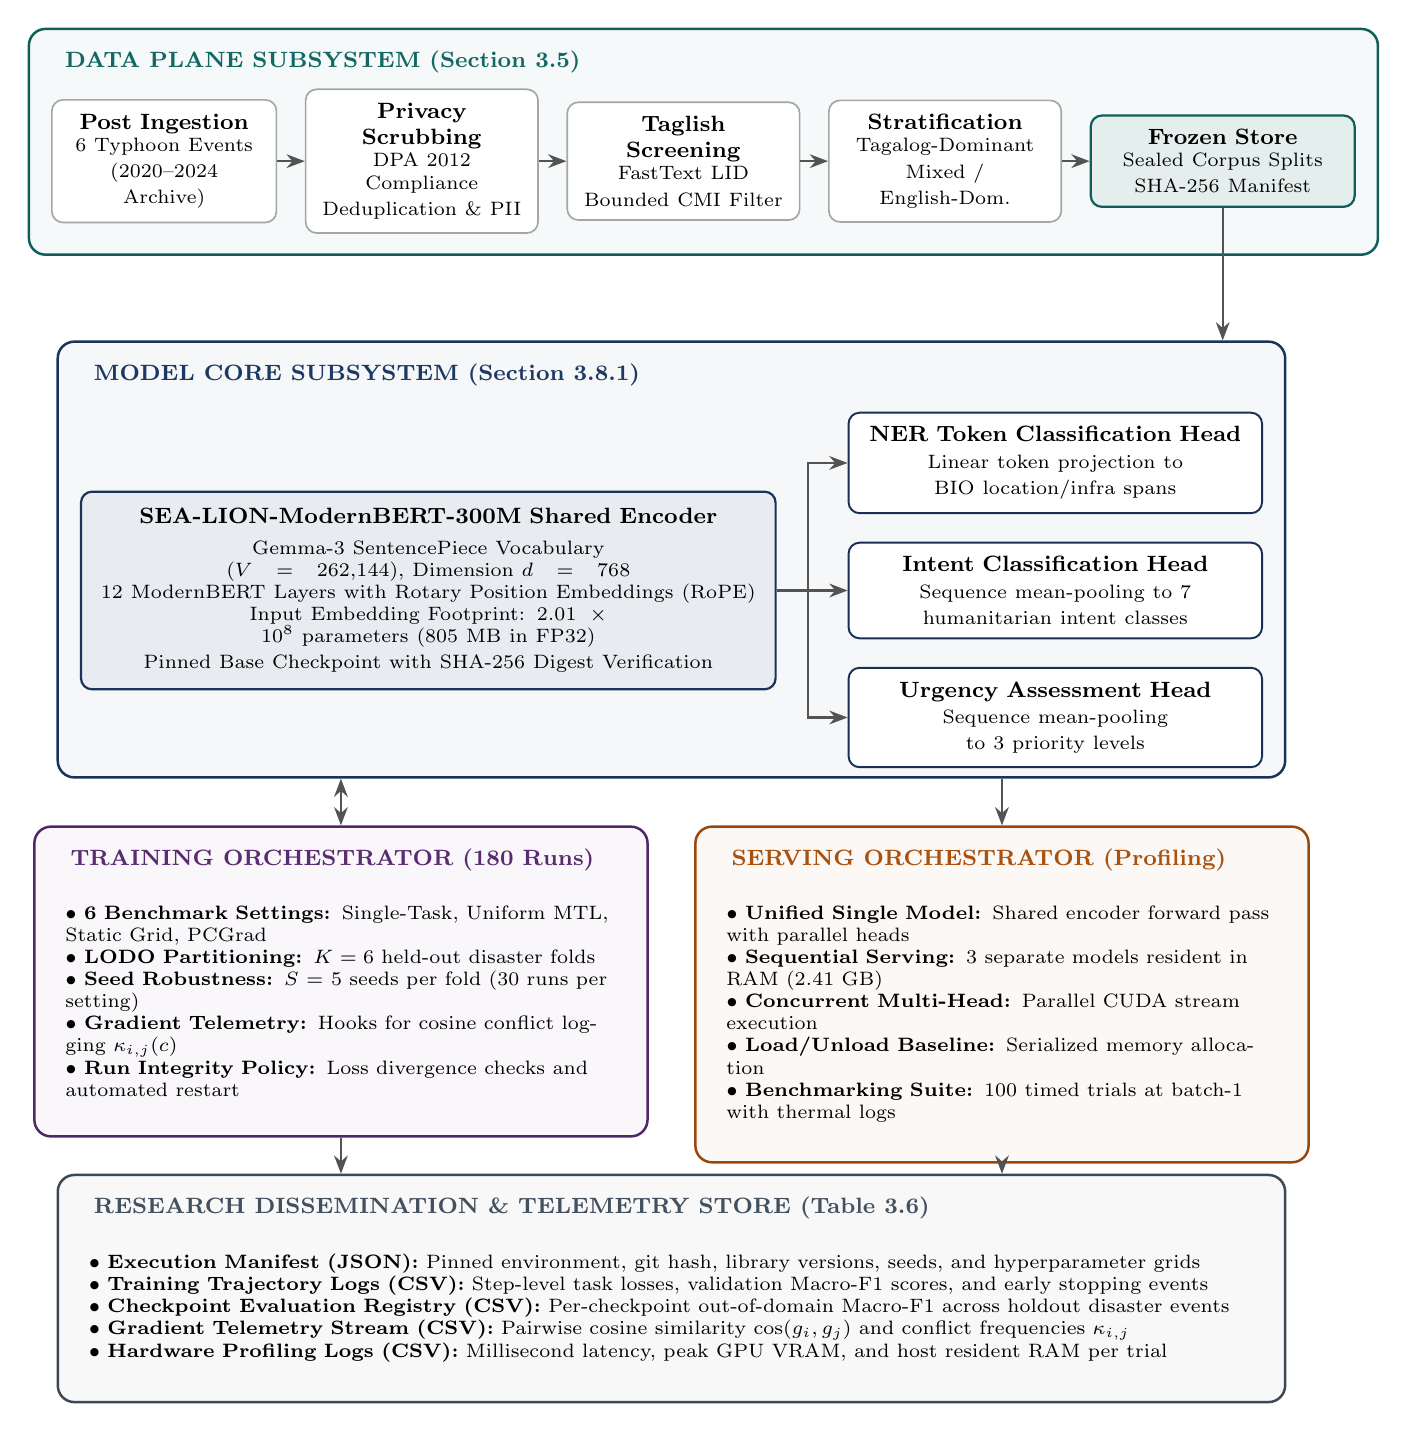
\begin{tikzpicture}[
    font=\small,
    >=Stealth,
    % Styles
    subbox/.style={
        draw=#1!85!black,
        fill=#1!4,
        rounded corners=6pt,
        line width=0.9pt
    },
    titlelabel/.style={
        font=\bfseries\footnotesize,
        text=#1!95!black,
        anchor=north west
    },
    proc/.style={
        draw=gray!70,
        fill=white,
        rounded corners=4pt,
        align=center,
        inner sep=5pt,
        font=\footnotesize,
        line width=0.6pt
    },
    store/.style={
        draw=datagreen!85!black,
        fill=datagreen!12,
        rounded corners=4pt,
        align=center,
        inner sep=5pt,
        font=\footnotesize,
        line width=0.8pt
    },
    corenode/.style={
        draw=modelblue!85!black,
        fill=modelblue!10,
        rounded corners=4pt,
        align=center,
        inner sep=6pt,
        font=\footnotesize,
        line width=0.8pt
    },
    headnode/.style={
        draw=modelblue!80!black,
        fill=white,
        rounded corners=4pt,
        align=center,
        inner sep=5pt,
        font=\footnotesize,
        line width=0.7pt
    },
    itemnode/.style={
        align=left,
        inner sep=3pt,
        font=\scriptsize
    },
    arrow/.style={
        ->,
        thick,
        draw=gray!65!black
    },
    biarrow/.style={
        <->,
        thick,
        draw=gray!65!black
    }
]

    % =========================================================================
    % 1. DATA PLANE SUBSYSTEM (Top Row)
    % =========================================================================
    \node[proc, text width=2.5cm] (dp1) {
        \textbf{Post Ingestion}\\
        \scriptsize 6 Typhoon Events\\
        \scriptsize (2020--2024 Archive)
    };

    \node[proc, right=0.35cm of dp1, text width=2.6cm] (dp2) {
        \textbf{Privacy Scrubbing}\\
        \scriptsize DPA 2012 Compliance\\
        \scriptsize Deduplication \& PII
    };

    \node[proc, right=0.35cm of dp2, text width=2.6cm] (dp3) {
        \textbf{Taglish Screening}\\
        \scriptsize FastText LID\\
        \scriptsize Bounded CMI Filter
    };

    \node[proc, right=0.35cm of dp3, text width=2.6cm] (dp4) {
        \textbf{Stratification}\\
        \scriptsize Tagalog-Dominant\\
        \scriptsize Mixed / English-Dom.
    };

    \node[store, right=0.35cm of dp4, text width=3.0cm] (dpstore) {
        \textbf{Frozen Store}\\
        \scriptsize Sealed Corpus Splits\\
        \scriptsize SHA-256 Manifest
    };

    \draw[arrow] (dp1) -- (dp2);
    \draw[arrow] (dp2) -- (dp3);
    \draw[arrow] (dp3) -- (dp4);
    \draw[arrow] (dp4) -- (dpstore);

    \begin{scope}[on background layer]
        \node[subbox=datagreen, 
              fit={(dp1) (dpstore) ([yshift=22pt]dp1.north) ([yshift=-8pt]dp1.south)}, 
              inner xsep=8pt] (databox) {};
    \end{scope}
    \node[titlelabel=datagreen] at ([xshift=10pt, yshift=-5pt]databox.north west) 
        {DATA PLANE SUBSYSTEM (Section 3.5)};

    % =========================================================================
    % 2. MODEL CORE SUBSYSTEM (Middle Section)
    % =========================================================================

    % Task Heads stacked cleanly without overlap
    \node[headnode, below=2.4cm of dp4, text width=4.9cm, xshift=1.4cm] (head_ner) {
        \textbf{NER Token Classification Head}\\
        \scriptsize Linear token projection to BIO location/infra spans
    };

    \node[headnode, below=0.35cm of head_ner, text width=4.9cm] (head_intent) {
        \textbf{Intent Classification Head}\\
        \scriptsize Sequence mean-pooling to 7 humanitarian intent classes
    };

    \node[headnode, below=0.35cm of head_intent, text width=4.9cm] (head_urgency) {
        \textbf{Urgency Assessment Head}\\
        \scriptsize Sequence mean-pooling to 3 priority levels
    };

    % Shared Encoder placed to the left, vertically centered with Intent head
    \node[corenode, left=0.9cm of head_intent, text width=8.4cm] (encoder) {
        \textbf{SEA-LION-ModernBERT-300M Shared Encoder}\\[3pt]
        \scriptsize Gemma-3 SentencePiece Vocabulary ($V = 262{,}144$), Dimension $d = 768$\\
        \scriptsize 12 ModernBERT Layers with Rotary Position Embeddings (RoPE)\\
        \scriptsize Input Embedding Footprint: $2.01 \times 10^8$ parameters ($805\text{ MB}$ in FP32)\\
        \scriptsize Pinned Base Checkpoint with SHA-256 Digest Verification
    };

    % Branching arrows from Encoder to Heads
    \draw[arrow] (encoder.east) -- ++(0.4,0) |- (head_ner.west);
    \draw[arrow] (encoder.east) -- (head_intent.west);
    \draw[arrow] (encoder.east) -- ++(0.4,0) |- (head_urgency.west);

    \begin{scope}[on background layer]
        \node[subbox=modelblue, 
              fit={(encoder) (head_ner) (head_urgency) ([yshift=22pt]head_ner.north) ([yshift=-8pt]encoder.south)}, 
              inner xsep=8pt] (modelbox) {};
    \end{scope}
    \node[titlelabel=modelblue] at ([xshift=10pt, yshift=-5pt]modelbox.north west) 
        {MODEL CORE SUBSYSTEM (Section 3.8.1)};

    % Flow from Frozen Corpus Store to Model Subsystem
    \draw[arrow] (dpstore.south) -- (dpstore.south |- modelbox.north);

    % =========================================================================
    % 3. EXECUTION ORCHESTRATORS (Bottom Left & Right)
    % =========================================================================

    % Training Orchestrator Box (Left)
    \node[itemnode, below=1.5cm of modelbox.south west, anchor=north west, text width=7.0cm] (traintext) {
        $\bullet$ \textbf{6 Benchmark Settings:} Single-Task, Uniform MTL, Static Grid, PCGrad\\
        $\bullet$ \textbf{LODO Partitioning:} $K = 6$ held-out disaster folds\\
        $\bullet$ \textbf{Seed Robustness:} $S = 5$ seeds per fold ($30$ runs per setting)\\
        $\bullet$ \textbf{Gradient Telemetry:} Hooks for cosine conflict logging $\kappa_{i,j}(c)$\\
        $\bullet$ \textbf{Run Integrity Policy:} Loss divergence checks and automated restart
    };

    \begin{scope}[on background layer]
        \node[subbox=trainpurple, 
              fit={(traintext) ([yshift=22pt]traintext.north) ([yshift=-8pt]traintext.south)}, 
              inner xsep=8pt] (trainbox) {};
    \end{scope}
    \node[titlelabel=trainpurple] at ([xshift=10pt, yshift=-5pt]trainbox.north west) 
        {TRAINING ORCHESTRATOR (180 Runs)};

    % Serving Orchestrator Box (Right)
    \node[itemnode, below=1.5cm of modelbox.south east, anchor=north east, text width=7.0cm] (servetext) {
        $\bullet$ \textbf{Unified Single Model:} Shared encoder forward pass with parallel heads\\
        $\bullet$ \textbf{Sequential Serving:} 3 separate models resident in RAM ($2.41\text{ GB}$)\\
        $\bullet$ \textbf{Concurrent Multi-Head:} Parallel CUDA stream execution\\
        $\bullet$ \textbf{Load/Unload Baseline:} Serialized memory allocation\\
        $\bullet$ \textbf{Benchmarking Suite:} 100 timed trials at batch-1 with thermal logs
    };

    \begin{scope}[on background layer]
        \node[subbox=serveorange, 
              fit={(servetext) ([yshift=22pt]servetext.north) ([yshift=-8pt]servetext.south)}, 
              inner xsep=8pt] (servebox) {};
    \end{scope}
    \node[titlelabel=serveorange] at ([xshift=10pt, yshift=-5pt]servebox.north west) 
        {SERVING ORCHESTRATOR (Profiling)};

    % Arrows between Model Core and Orchestrators
    \draw[biarrow] (modelbox.south -| trainbox.center) -- (trainbox.north);
    \draw[arrow] (modelbox.south -| servebox.center) -- (servebox.north);

    % =========================================================================
    % 4. TELEMETRY & LOGGING PIPELINE (Bottom Full Width)
    % =========================================================================
    \node[itemnode, below=1.2cm of $(trainbox.south)!0.5!(servebox.south)$, anchor=north, text width=14.8cm] (logtext) {
        $\bullet$ \textbf{Execution Manifest (JSON):} Pinned environment, git hash, library versions, seeds, and hyperparameter grids\\
        $\bullet$ \textbf{Training Trajectory Logs (CSV):} Step-level task losses, validation Macro-F1 scores, and early stopping events\\
        $\bullet$ \textbf{Checkpoint Evaluation Registry (CSV):} Per-checkpoint out-of-domain Macro-F1 across holdout disaster events\\
        $\bullet$ \textbf{Gradient Telemetry Stream (CSV):} Pairwise cosine similarity $\cos(g_i, g_j)$ and conflict frequencies $\kappa_{i,j}$\\
        $\bullet$ \textbf{Hardware Profiling Logs (CSV):} Millisecond latency, peak GPU VRAM, and host resident RAM per trial
    };

    \begin{scope}[on background layer]
        \node[subbox=logslate, 
              fit={(logtext) ([yshift=22pt]logtext.north) ([yshift=-8pt]logtext.south)}, 
              inner xsep=8pt] (logbox) {};
    \end{scope}
    \node[titlelabel=logslate] at ([xshift=10pt, yshift=-5pt]logbox.north west) 
        {RESEARCH DISSEMINATION \& TELEMETRY STORE (Table 3.6)};

    % Arrows from Orchestrators down to Log Store
    \draw[arrow] (trainbox.south) -- (trainbox.south |- logbox.north);
    \draw[arrow] (servebox.south) -- (servebox.south |- logbox.north);

\end{tikzpicture}
\end{document}
